\documentclass{article}
\usepackage{tikz}
\usepackage{amsmath}
\usepackage{bm}
\usepackage{scalerel}
\usepackage{pgfplots}
\usepackage{mathpazo}
\pgfplotsset{width=7cm,compat=1.8}
\usetikzlibrary{patterns}
\usetikzlibrary{arrows,shapes,calc}
\usetikzlibrary{external}
\tikzset{external/system call={pdflatex \tikzexternalcheckshellescape -halt-on-error
        -interaction=batchmode -jobname "\image" "\texsource" && %  or ;
pdftops -eps "\image".pdf}}
\tikzexternalize


\begin{document}


	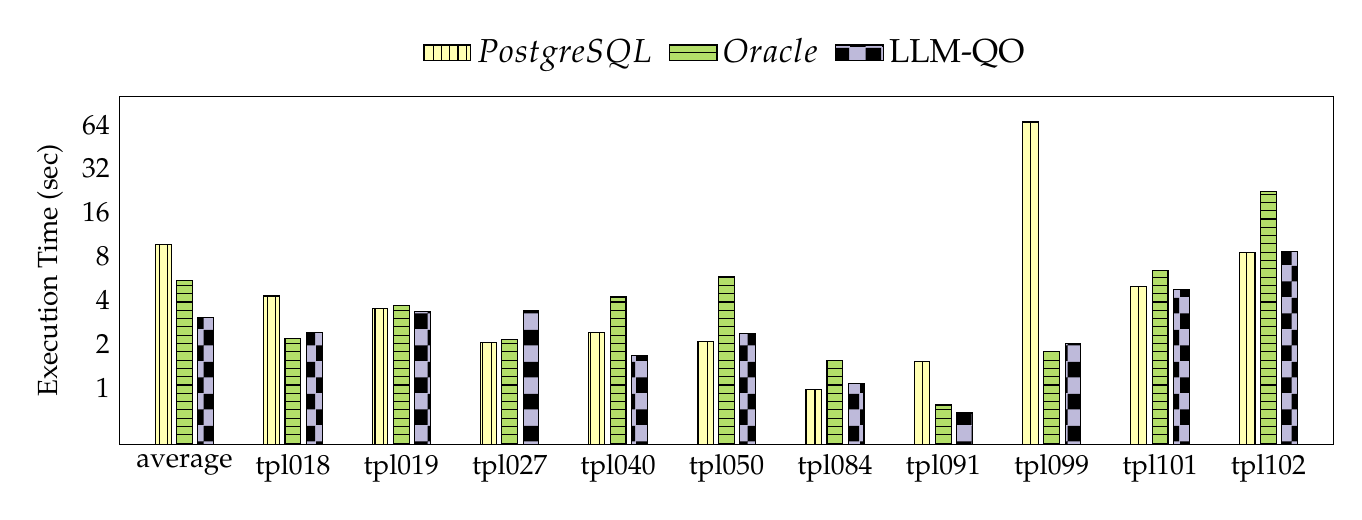
\begin{tikzpicture}
	\definecolor{lssfre}{HTML}{fccde5}
	\definecolor{lssemb}{HTML}{bc80bd}
	\definecolor{dann}{HTML}{bebada}
	\definecolor{fauce}{HTML}{bdfcc9}
	\definecolor{mixup}{HTML}{fb8072}
	\definecolor{groupdro}{HTML}{80b1d3}
	\definecolor{mask}{HTML}{fdb462}
	\definecolor{cset}{HTML}{b3de69}
	\definecolor{order}{HTML}{8dd3c7}
	\definecolor{erm}{HTML}{ffffb3}
	\definecolor{coral}{HTML}{d9d9d9}
	\definecolor{gflow}{HTML}{778899}
	\definecolor{BNN}{HTML}{92b6d5}
	\definecolor{MCD}{HTML}{d9d9d9}
	\centering
	\begin{axis}[
	ybar, %axis on top,
	height=6cm, width=17cm,
	bar width=0.2cm,
	tick align=inside,
	%enlarge y limits={value=.1,upper},
	ymin=0, ymax=100, 
	tickwidth=0pt,
	ymode=log,
	log origin=infty,
	enlarge x limits=true,
	legend style={
		draw=none,
		at={(0.5, 1.2)},
		anchor=north,
		legend columns=3,
		/tikz/every even column/.append style={column sep=0.15cm}
	},
	ylabel={Execution Time (sec)},
	ytick={1, 2, 4, 8, 16, 32, 64},
	yticklabels={1, 2, 4, 8, 16, 32, 64},
	xmin=1, xmax = 29,
	xtick={0, 3, 6, 9, 12, 15, 18, 21, 24, 27, 30},
	xticklabels={average, tpl018, tpl019, tpl027, tpl040, tpl050, tpl084, tpl091, tpl099, tpl101, tpl102},
	%nodes near coords,
	%nodes near coords style={font=\tiny}, 
	%point meta = explicit,
	%point style={font=\scriptsize}, 
	%xlabel={Dataset},
	%xlabel style={yshift=1ex},
	%xlabel style={font=\large},
	%symbolic x coords={
	%	Facebook, Gowalla, WikiConflict, Google, DBLP, Berkstan, Youtube, Petster, Flickr,
	%Indochina },
	%xtick=data,
	]
\vspace{-4mm}

	% PostgreSQL
 	\addplot [ybar, fill=erm, postaction={pattern=vertical lines}, area legend] coordinates {
(0, 9.64)
(3, 4.27)
(6, 3.48)	
(9, 2.05)
(12, 2.38)	
(15, 2.07)
(18, 0.97)
(21, 1.52)
(24, 67.04)	
(27, 4.94)
(30, 8.49)	
    };
        
    
    % Oracle
 	\addplot [ybar, fill=cset, postaction={pattern=horizontal lines}, area legend] coordinates {	
(0, 5.45)
(3, 2.17)
(6, 3.68)	
(9, 2.14)
(12, 4.20)	
(15, 5.79)
(18, 1.54)	
(21, 0.76)
(24, 1.78)	
(27, 6.35)
(30, 22.18)		
    };

    

  
    
    % LLM-QO(DPO)
 	\addplot [ybar, fill=dann, postaction={pattern=checkerboard}, area legend] coordinates {	
(0, 3.02)
(3, 2.38) % imdb 
(6, 3.33)	% tpcds
(9, 3.4) % imdb 
(12, 1.66)	% tpcds
(15, 2.35) % imdb 
(18, 1.07)	% tpcds
(21, 0.67)
(24, 2.00)	
(27, 4.71)
(30, 8.64)	
    };





	%\LLMQO (\QIT), \LLMQO (\QDPO) and \LLMQO (\QDPO)$^{+}$
    
	\legend{
		    \large ${\sl PostgreSQL}$,
		    \large ${\sl Oracle}$,
		     \large {\text{LLM-QO}},
		     %		    \large $\texttt{OrderEmb}$,
%	   	    \large $\texttt{NeuroCard}$,
%		    \large $\texttt{Postgres}$,
%			\large $\texttt{SQL Server}$,
%		    \large $\texttt{GP-RBF}$
	        }
	\end{axis}
	\end{tikzpicture}


\end{document}
